\documentclass[12pt]{article}
\usepackage[margin=2.5cm]{geometry}
\usepackage{enumerate}
\usepackage{amsfonts}
\usepackage{amsmath}
\usepackage{fancyhdr}
\usepackage{amsmath}
\usepackage{amssymb}
\usepackage{amsthm}
\usepackage{mdframed}
\usepackage{graphicx}
\usepackage{subcaption}
\usepackage{adjustbox}
\usepackage{listings}
\usepackage{xcolor}
\usepackage{booktabs}
\usepackage[utf]{kotex}
\usepackage{hyperref}

\definecolor{codegreen}{rgb}{0,0.6,0}
\definecolor{codegray}{rgb}{0.5,0.5,0.5}
\definecolor{codepurple}{rgb}{0.58,0,0.82}
\definecolor{backcolour}{rgb}{0.95,0.95,0.92}

\lstdefinestyle{mystyle}{
    backgroundcolor=\color{backcolour},
    commentstyle=\color{codegreen},
    keywordstyle=\color{magenta},
    numberstyle=\tiny\color{codegray},
    stringstyle=\color{codepurple},
    basicstyle=\ttfamily\footnotesize,
    breakatwhitespace=false,
    breaklines=true,
    captionpos=b,
    keepspaces=true,
    numbers=left,
    numbersep=5pt,
    showspaces=false,
    showstringspaces=false,
    showtabs=false,
    tabsize=1
}

\lstset{style=mystyle}

\pagestyle{fancy}
\renewcommand{\headrulewidth}{0.4pt}
\lhead{Hyungmo Gu}
\rhead{CSC369 Week 2 Notes}

\begin{document}
\title{CSC369 Week 2 Notes}
\author{Hyungmo Gu}
\maketitle

\section{System Calls}

\bigskip

\begin{itemize}
    \item Bootstraping
    \begin{itemize}
        \item Bootstraping

        \begin{center}
        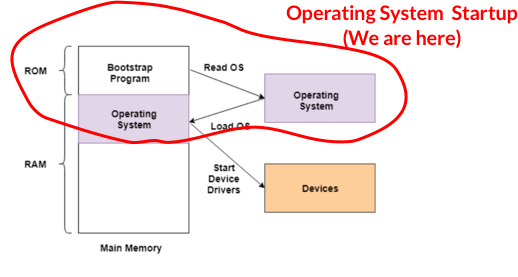
\includegraphics[width=\linewidth]{images/week_2_notes_1_3.png}
        \end{center}


        \begin{itemize}
            \item executes \textbf{Bootstrap Program}
            \begin{itemize}
                \item is the first code that runs when the computer system is started
            \end{itemize}
            \item Entire operating system depnds on the bootstrap program to work
            correctly
            \item Locates and loads kernel (code of operating system) onto RAM
            \begin{itemize}
                \item kernel = code of the operating system
                \item kernel is in HDD
                \item bootstrap program finds and loads it RAM
            \end{itemize}
            \item Bootstrap program is in ROM
        \end{itemize}

        \item ROM
        \begin{itemize}
            \item is called \textbf{read-only-memory}
            \item Is also called \textbf{BIOS chip} (Basic Input/Output System)
            \item is non-volatile
            \item Knows how to access simple hardware devices
            \begin{itemize}
                \item i.e. Disk, keyboard, display
            \end{itemize}

            \item is stored in motherboard

            \begin{center}
            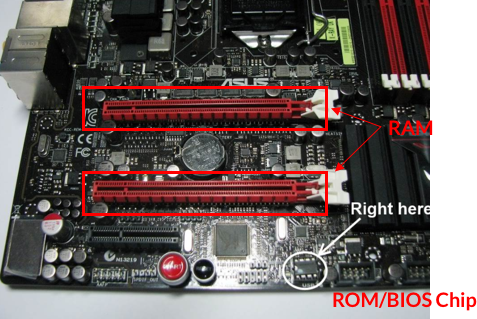
\includegraphics[width=0.8\linewidth]{images/week_2_notes_1_2.png}
            \end{center}
        \end{itemize}
    \end{itemize}

    \item Operating System Startup

    \begin{center}
    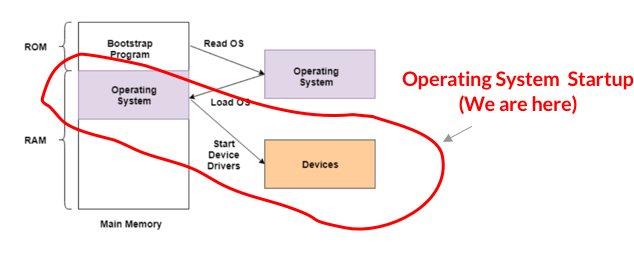
\includegraphics[width=\linewidth]{images/week_2_notes_1_4.png}
    \end{center}

    \begin{itemize}
        \item Initializes OS
        \begin{itemize}
            \item Initialize internal data structures
            \item Create first process
            \item Switch mode to user and start runing first process
            \item Wait for something to happen
        \end{itemize}
    \end{itemize}

    \item Memory Layout
    \item Requesting OS Services
    \item Boundary Crossings
    \item System Calls for Process Management
    \item System Calls for File Management

\end{itemize}

\end{document}